


\documentclass[10pt,journal,compsoc]{IEEEtran}

\ifCLASSOPTIONcompsoc
  % IEEE Computer Society needs nocompress option
  % requires cite.sty v4.0 or later (November 2003)
  \usepackage[nocompress]{cite}
  \usepackage{graphicx}
\else
  % normal IEEE
  \usepackage{cite}
\fi

\ifCLASSINFOpdf
  % \usepackage[pdftex]{graphicx}
  % declare the path(s) where your graphic files are
  % \graphicspath{{../pdf/}{../jpeg/}}
  % and their extensions so you won't have to specify these with
  % every instance of \includegraphics
  % \DeclareGraphicsExtensions{.pdf,.jpeg,.png}
\else
  % or other class option (dvipsone, dvipdf, if not using dvips). graphicx
  % will default to the driver specified in the system graphics.cfg if no
  % driver is specified.
  % \usepackage[dvips]{graphicx}
  % declare the path(s) where your graphic files are
  % \graphicspath{{../eps/}}
  % and their extensions so you won't have to specify these with
  % every instance of \includegraphics
  % \DeclareGraphicsExtensions{.eps}
\fi
\hyphenation{op-tical net-works semi-conduc-tor}


\begin{document}

\title{Effectiveness of adversarial example generation methods in image recognition deep learning framework}


\author{Rafael Carvalhaes Possas, University of Sydney, Australia}

\markboth{University of Sydney, Australia, October~2016}%
{Shell \MakeLowercase{\textit{et al.}}: Image recognition: Adversarial Examples in Deep Learning}



\IEEEtitleabstractindextext{%
\begin{abstract}
Computer Image recognition have become increasingly popular nowadays due to the increase in demand for wearables, smartphones and any kind of device with attached cameras. Camera sensors and processing power received considerable improvements across the years and have reached a point where sophisticated algorithms are able to run on these devices and provide state of the art computer vision performance. Yet little is known about how the developed techniques can learn and generalize their results on such tasks. One could create perturbation on a specific image and feed it into these algorithms in order to change the output of the prediction. This new image is known as Adversarial. This study focuses on identifying the relationship between the classification confidence on a deep learning network and two different methods for adversarial creation: Fast Gradient Sign and Iterative Gradient Sign
\end{abstract}

% Note that keywords are not normally used for peerreview papers.
\begin{IEEEkeywords}
Deep Learning, Computer Vision, Machine Learning, Adversarial examples.
\end{IEEEkeywords}}


% make the title area
\maketitle

\IEEEdisplaynontitleabstractindextext
\IEEEpeerreviewmaketitle



\IEEEraisesectionheading{\section{Introduction}\label{sec:introduction}}

\IEEEPARstart{R}{ecent} advancements in computational power and the development of Deep Learning techniques helped to popularize
the use of Computer Vision. Deep Learning algorithms are better represented through Convolutional Neural
Networks where several layers of neurons are connected and each of these represent deep characteristics of the input
data.

Neural Networks have been the underlying foundation of such algorithms. These are able to represent highly non-linear and complex mathematical problems and, thus,  able to work very well on datasets with an increased number of dimensions. Machine Learning systems are becoming ubiquitous and, therefore, require to be not only very accurate but also robust to any kind of attack. Methods for exploiting vulnerabilities have been found and should become a major concern for those using these algorithms

Several machine learning models, Convolutional Neural Networks included, can misclassify adversarial images \cite{goodfellow2014}\cite{papernot2016transf}\cite{goodfellow2016}\cite{szegedy2013}. Such examples are usually created through applying small intentional perturbations to each pixel in a way that the classifier outputs the incorrect answer, while, for human beings, these perturbations do not affect the overall understanding of the desired class in most cases.

Lets say there is a machine learning system \textit{A} and an input image \textit{I}. Initially, this input sample is correctly classified by some machine learning system (e.g. A(I) = true label). It is then, possible to create an Adversarial Sample $\alpha$ from our image such as our machine learning system yields a wrong label output when the image is fed into the system (e.g. A($\alpha$) = false label).

Adversarial examples pose some relevant security threats for practical machine learning systems. The wrong use of these techniques can lead to bad outcomes and should, therefore, be avoided. Since the first development of the Fast Gradient Sign by Goodfellow et al. (2014), some more relevant work have been developed in order to reveal insights about the adversarial nature. For instance, Szegedy et al. (2014) showed that an adversarial example that was initially crafted to attack a specific model, could also be used to attack other similar models.These and other properties of deep learning algorithms highlights that such systems knowledge is transferable and, therefore, would make these systems more vulnerable to these attacks.

The Fast Gradient sign method depends on gradient information in order to create the perturbations of the input image. This information can be obtained by either running the backpropagation on the desired target network with the image as an input or to train a network by querying the target with some chosen sample set and then using this new network to retrieve gradient information. Both methods can yield significant error rates \cite{goodfellow2014}\cite{papernot2016transf} for adversarials and, thus, should be considered an imminent threat for deep learning systems.

The resulting new label of an adversarial image can sometimes be driven by some desired class label. For instance, one could use image A label in order to make image B classification output to be closer to class A output. However, this is not always true as it depends on intrinsic network configuration and image characteristics. For this work, two methods for choosing the perturbation type will be used. The least likely method, where the output label on the top 5 results with the lower confidence will be chosen as the label on which the gradient information will be extracted and the inverse method, where the true image label gradient will be used to make the image looks less likely itself.

Label prediction confidence is another factor to consider when evaluating Softmax CNN networks. Anecdotal evidence claims that higher confidence prediction makes an image prediction less likely to be perturbed by adversarial methods. This work will test images with three different confidence intervals (High, Medium and Low) along with both iterative and fast gradient sign and the aforementioned perturbation types (least likely class and inverse method).

This specific scenario has not been yet been addressed by current research community and can be valuable to help one to interpret and understand not only the underlying behaviour of a Deep Learning algorithm but also to use adversarial methods to improve robustness of these algorithms. 

The use of image miss-classification through adversarial examples can help to answer some DNNs behavioral questions. Firstly, how likely images with high, medium and low confidence are affected by methods like the Fast Gradient Sign and the Iterative Gradient Sign when both inverse and least likely perturbation method is used \cite{goodfellow2014}\cite{goodfellow2016}. Secondly, which of these methods can successfully generate examples that yields wrong labels when fed into state of the art DNNs. Finally, it is important to identify the relationship between the aforementioned factors in order to provide insights of how these so called, complex algorithms, are generalizing their results. By exploring DNNs weaknesses we intend to give a different perspective on understanding deep learning algorithms performance.

\section{Related Work}
\label{sec:related_work}
Since the discovery of the gradient sign method on Goodfellow et al (2014), research in adversarial methods have been growing considerably. Studies range from using unrecognizable images like Nguyen et al. (2015) \cite{nguyen2015} to the use of images in the physical world \cite{goodfellow2016}. Adversarial crafting based on gradient sign is highly dependent on the network internal knowledge, more specifically, the gradient vector \cite{papernot2016transf}. As it was mentioned on Papernot et al. (2016), knowledge transfer is an interesting property of differentiable machine learning systems, and definitely can be learned through simple queries to the system in which the gradient wants to be extracted. This method is known as black box attack and it was the object of study also in \cite{papernot2016}. All of these techniques poses threat to the current state of computer vision algorithms, as the wrong use of such can yield unwanted/negative outcomes for the users of such systems.
\section{Problem Statement}
\label{sec:research_question}

Adversarial experimentation have contributed to a better understanding of the underlying mathematical calculations on CNNs. For instance, by understanding where a gradient perturbation happens it is possible to visualize which pixels in an image are more relevant, and, therefore, create an intuition of what the computer is actually "seeing" \cite{lowd2005}. Most methods are highly dependent on the Fast Gradient Sign developed. However, the performance of these algorithms on images with different levels of classification confidence and using different gradients is still unanswered. Both Fast Gradient Sign and Iterative Sign methods should be highlighted and compared in this work alongside the impact of different image classification confidence and perturbation methods on the overall adversarial performance.

$$ C(x + \delta)\approx C(x) + \delta * \nabla C$$

The Gradient Sign equation shows that the perturbation is one such that it emphasizes the pixels in the image with the highest importance, so the resulting perturbation can likely lead to a misclassified result. By using the \textit(sign) function of the gradient, it is assured that the value will grow linearly with the number of the dimensions \cite{goodfellow2014}. The result of many small pixel changes is likely to generate an image with a wrong label in the network output. The gradient information can be generated from a arbitrary image or from a specific label of any image. For instance, one could use the image true label to generate the gradient vector $\nabla$C and, thus perturb the pixels in the opposite direction, making the image look less likely itself. On the other hand, the lowest prediction of the top 5 softmax layer could also be used to deviate the original label towards the new selected weaker label prediction.

Anecdotal evidence claims that higher levels of classification confidence provides robustness against adversarial perturbation methods. However, the overall result could depend on the type of perturbation applied to the input image and what gradient information would be used as the perturbation vector $\nabla$C. For instance, the iterative gradient sign relies on small perturbation and gradient direction optimization through iteratively small steps while the fast gradient sign provides a one time only big perturbation to every pixel. Different gradients $\nabla$C would need different values for the $\delta$ in the sign method and therefore are very hard to compare. On this way, the gradient used in this paper is based on the image gradient with two different scenarios. By using the Least Likely Method and Inverse method, one would have less arbitrary gradients as they would have in all cases a closer relationship with the image being perturbed.The main focus is to understand how different gradient sign methods compare when using related gradient information and images with different classification confidence levels.

Recent research efforts on Deep Learning have been devoted to visualizing the image features detected by each of the layers of a network. In convolutional networks, the initial layers are usually responsible for detecting simple features (edges, combinations of edges etc) while later layers can detected higher-order combinations of features \cite{yosinski2015understanding}. Even that this understanding is important, it will not be the focus of this work, however, results will help understanding possible weak spots of networks and the factors leading to the success of gradient sign methods.

\section{Methods and Design}
\label{sec:methods}
In the last years, object detection classification capabilities have dramatically improved due to advances in not only deep learning and convolutional networks but also to the availability of fine tuned datasets as the ImageNet \cite{deng2009imagenet} used in most of the ILSVRC competitions. One of the major issues with image and pattern recognition until the release of such dataset was how the data could be harnessed and organized in order to provide a resourceful asset for training networks.

The availability of ImageNet pre-trained networks through popular software packages have been increasingly helpful for research developments. The network used on this work is based on the Inception V3 model as described and explained in Szegedy et al (2015) \cite{szegedy2015going}. The main idea of this architecture is to provide optimized local sparse structure of vision networks. In other words, the network will be built from convolutional blocks or "Inception modules" stacked on top of each other capable of detecting both fined grained and abstract features of the input images. \cite{szegedy2015going}.

The sample set used is composed of 1.500 total images classified in three equally distributed levels of confidence. Considering the top-5 results of a Softmax layer, images were divided into buckets of high, medium and low confidence. High confidence images were those were the right prediction was the top-1 result with 30\% or more of confidence associated to the label. Medium confidence should have the top-1 result sitting between 15\% and 30\% while everything below 15\% would be seen as low confidence.

Generating the gradient in which the perturbation would be based is crucial for having successful adversarial creation \cite{goodfellow2016}. The gradient can be seen as the direction of which the combination of pixels in an image are pointing into the high-dimensional space. Therefore, using the own image gradient would result in perturbations that are in a way related to the current chosen direction. Two gradients were chosen for creating perturbations of the training set. Firstly, the true image label or top-1 result was used as the gradient but the the gradient vector was subtracted from each pixel, instead of being added. This results in making the image to look less likely itself, and the method will be called the Inverse Gradient Sign. Secondly,  the perturbation was also generated through the gradient of the top-5 prediction of the softmax layer, which in other words means making our image to look like the selected label, this will be called the Least Likely Method. It is important to note that these two methods were chosen in order to make the gradient sign generation less arbitrary as the gradient used is individually correlated to each specific image.

The different methods used to generate adversarial examples will vary on how they apply gradient perturbation on each pixel of the input image. The simplest method to generate these images is known as Fast Method \cite{goodfellow2014}. The motivation behind the method is to linearize the cost function solving for the perturbation that maximizes the cost. The second method, known as iterative method described in Goodfellow et al. 2016 \cite{goodfellow2016} is a straightforward variation of the fast method. The noise is applied multiple times with small step size, resulting in slower and more fine tuned pixel perturbation.

The experiments were based on testing all the three aforementioned combinations (confidence, gradient perturbation and methods) on the entire dataset (1.500 images).The aim is to understand not only how they compare but also possible factors leading to the success of adversarial methods and perturbation.
\section{Results}
\label{sec:results}

Least Likely methods had a lower overall impact into the image, resulting into lower error rates and, therefore, into less miss-classified examples. As the gradient used has a lower numerical significance, images running on the fast method would not have enough noise being added as one single iteration would add a very small numerical perturbation. Besides, lower confidence level images seemed to be more vulnerable to perturbations. This can be explained by understanding that in the high dimensional space, the gradient vector would be pointed almost equally at more than one direction, thus, perturbations of even smaller magnitudes would already have an impact on the classification outcome.

On the other hand, the inverse technique had a lower gap between fast and iterative methods and seemed to be more efficient for adversarial creation. The same aforementioned analogy applies in here, higher magnitude gradients can generate higher perturbations and, thus, achieve better error rates. Making an image to look less likely itself is the same as inverting the direction of the gradient and optimizing pixels according to this new direction. Images level of confidence play similar role in here, as the higher the confidence, the less likely it is to generate a successful adversarial. For instance, lower confidence images were able to achieve 91\% top-1 error rate with the iterative/inverse techniques.
\begin{table}[h!]
\centering
	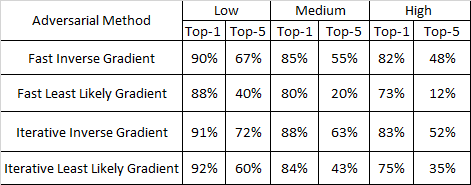
\includegraphics[scale=0.7]{results.png}
\caption{Error rates for all combinations}

\end{table}

The results show that it might be more difficult to completely remove the image from the top-5 predictions as it would need way more noise being added to pixels in order to completely wipe the original label from the top-5 softmax results. This shows that CNNs are really learning important image characteristics and combined pixel variance as it takes more effort to disturb the learned pattern. Both low/medium confidence images and inverse perturbation methods play a major role on the overall performance of adversarial generation. At the same time, the addition of noise in small steps in many iterations is also more efficient, as the direction of the gradient is optimized by a small factor on each step.
% Table generated by Excel2LaTeX from sheet 'Sheet1'


\section{Conclusion}
Deep Learning perturbations can be seen as generative models that exploits the networks spaces where the posterior distribution does not have considerable probability mass, and , thus, creates perturbations that can completely change the output label. Methods for generating these so called adversarial examples are  more effective when the resulting confidence level is low, the gradient used is highly correlated with the current image and the perturbations are done in small optimized steps at a time. These methods should be considered in regularization techniques of systems where these attacks are likely to be avoided. In future work we expect that different methods/parameters could be tested in order to explore further the adversarial characteristics that can help in the development of regularization techniques.


% Can use something like this to put references on a page
% by themselves when using endfloat and the captionsoff option.
\ifCLASSOPTIONcaptionsoff
  \newpage
\fi

\pagebreak
\bibliographystyle{IEEEtran}
\bibliography{ref}

% that's all folks
\end{document}


